
L'exemple du menu étant simple et parlant, nous montrerons comment nous avons pensé 
ce module. Dans un menu, il y a des boutons. Donc il faut un objet Menu\footnote{De manière à être 
utilisable dans d'autres programmes, ou pouvoir faire plusieurs menus}, et un objet Bouton. Un Bouton est un objet affiché à l'écran, il faut donc le faire hériter de Rectangle, un objet Menu a une position sur l'écran, il faut donc aussi qu'il hérite de Rectangle.

De cette manière on a maintenant des classes comme ceci :
\begin{figure}[H]
	\centering
	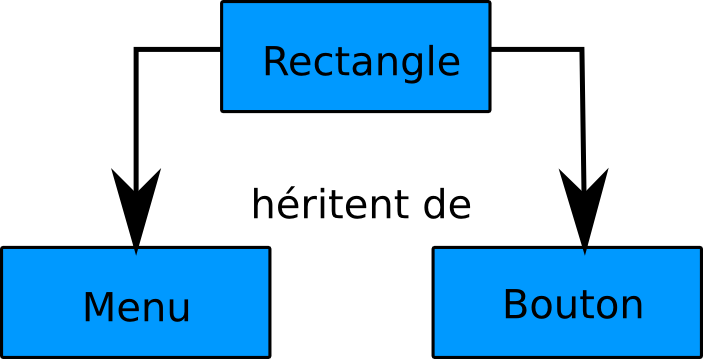
\includegraphics[width=26em]{Images/heritage_menu.png}
	\caption{Représentation de l'héritage des classes}
\end{figure} 
  
\subsection{Bouton}
	Bouton est une classe qui hérite de Rectangle, mais elle apporte son lot de nouveautés, à savoir tout ce qui est relatif au bouton : 
	\begin{itemize}
		\item une image pour le bouton normal
		\item une image pour le bouton activé
		\item une variable pour savoir si le bouton est activé
		\item une variable de type ennumération\footnote{Voir annexe \ref{DefEnum} sur les énnumération, qui parle du menu en exemple} pour savoir l'action qu'il entraine
	\end{itemize}
	
	Le bouton lui-même n'a pas vraiment de fonctions, tout le code se trouvera dans le gestionnaire des boutons, le Menu. Mais avant de parler du menu, il faut définir les actions, or nous ne savons pas encore lequelles il y aura, nous allons donc créer une énnumération, qui sera traitée dans la boucle des évènements. Ajouter une action demandera d'ajouter un item à l'énumération, et un traitement de cet item dans la boucle évènementielle.
	
\subsection{Menu}
	Le menu gère les boutons, son code n'est pas aussi complexe qu'on pourrait se l'imaginer, il contient un tableau de boutons, une fonction «~affiche~» qui affiche le menu et une fonction «~recupBouton~» qui retourne le bouton à la position du curseur.
	
	La seule difficulté réside dans le fait de dessiner correctement les boutons, et au bon endroit. Pour cela il faut savoir que l'écran de la SDL se comporte comme un repère orthonormé, à ceci près qu'il a pour origine le coin haut gauche de la fenêtre, et que son axe des Y est inversé par rapport aux graphiques habituels : 
	
	Après ça, il faut aussi savoir que le menu a une position, donc quand on place un Bouton, il faut le placer en fonction de la position du menu, et en fonction de la taille d'un Bouton. La méthode suivante est utilisée : 
	« $boutons.push(new Bouton (image,action, TAILLLE_BOUTON * numero_bouton + menu.x , menu.y,image_activé));$ ». Ce code se suffit, quand on crée un bouton, on lui donne deux images, une action, et la position du bouton vaut celle de la simulation, plus $N$ fois la largeur d'un bouton en $x$, en fonction du numéro du bouton.
	
	C'est bon, nous avons un menu fonctionnel, reste à connecter tout cela avec la boucle évènementielle et c'est terminé. Nous ne parlerons pas de la boucle évènementielle, car elle est en réalité simple. Globalement elle demande si le curseur a cliqué, si oui où. Après elle regarde sur quelle partie du programme le curseur est positionné, et un système de conditions décide de ce qu'il faut faire. Ce code n'est pas intéressant, simplement parce que c'est une suite de conditions imbriquées sans grande complexité.

